\section{Introduction}
\label{sec:intro}
Evaluating a model on a benchmark suite is expensive, and public leaderboards already hold the scores of hundreds of models on dozens or hundreds of benchmarks.
An evaluator with a new model and room for only $k$ benchmark runs faces three questions: which $k$ benchmarks to run, how to infer the scores on the other $N-k$, and how large $k$ must be before the inference is good enough.
Existing work shrinks the items inside one benchmark \citep{polo2024tinybenchmarks,vivek2024anchor,kipnis2024metabench}, measures how benchmarks agree \citep{perlitz2024benchbench}, or predicts scores from scale and model family \citep{ruan2024observational,polo2024sloth}; to our reading, none of them asks which whole benchmarks to run on a new model, nor how many.

We study this cold-start problem on the leaderboard score matrix itself.
Our reading of it is Bayesian experimental design on a latent-factor model: the posterior of a few latent capabilities given the $k$ scores run gives the prediction, a closed-form greedy gain chooses the benchmarks, and the posterior covariance forecasts the error and yields a stopping rule for $k$.
Gaussian sensor placement and the factor algebra are standard \citep{krause2008nearoptimal,das2011submodular}; we claim none of it as new.
The contribution is the combination with a protocol and with evidence that shows where it holds and where it does not.

\begin{figure}[t]
\centering
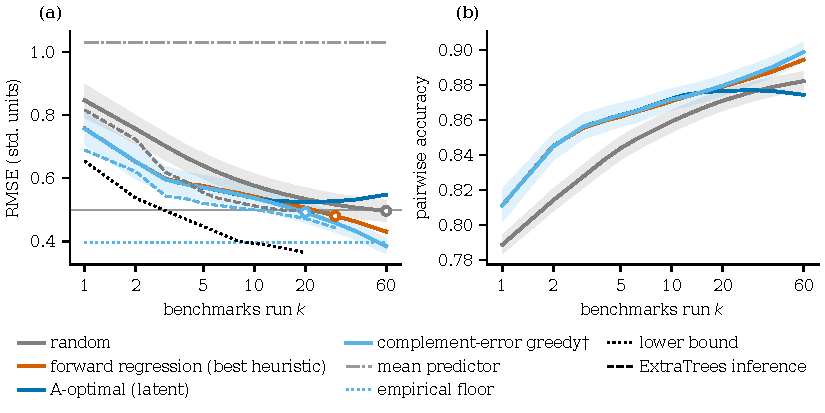
\includegraphics[width=\textwidth]{figures/f1.pdf}
\caption{A few benchmarks remove most of the error, but a tight tolerance needs many more. MTEB block A1 (103 models, 202 benchmarks), factor-posterior inference. (a) RMSE in standard-deviation units against the number of benchmarks run $k$: random choice, the A-optimal criterion, the complement-error greedy$^\dagger$ ($^\dagger$: added after a pilot) and forward regression, the best heuristic; bands: 95\% intervals; dashed: the same random and complement-error selections with ExtraTrees inference (no such curve in (b)); open circles mark the first grid $k$ with RMSE $\le0.5$. Dotted: the lower bound of Proposition~\ref{prop:floor} and the empirical floor (each benchmark predicted from all others), references not bounds. (b) Pairwise accuracy of ``which history models does the new model beat''.}
\label{fig:f1}
\end{figure}

\paragraph{Contributions.}
\begin{itemize}
\item \emph{A protocol} for sparse, non-stationary leaderboards in which every fitted quantity uses history rows only, a test model is scored on benchmarks it has actually been run on, and random, temporal and family-held-out splits are compared (Section~\ref{sec:setting}).
\item \emph{Theory with its checks.} An error decomposition, a floor on the error of every selector, a water-filling law for the achievable curve, and a conjecture for the effect of finite history from spiked-covariance theory, tested on synthetic matrices where the truth is known and on real ones; the closed-form forecast is accurate with known parameters and optimistic when fitted, and our finite-history correction does not improve on the plug-in forecast (Sections~\ref{sec:theory}, \ref{sec:experiments}).
\item \emph{An empirical map} of when few benchmarks suffice, with decision metrics beside RMSE, nonlinear imputers as the accuracy reference, and the effect of temporal and family shift.
\end{itemize}

\paragraph{What we find.}
On the complete MTEB block (103 models, 202 tasks), three benchmarks chosen by the model cut the RMSE from 1.03 (the history mean) to 0.60 standard deviations, $28\%$ below the MSE of three random ones (Figure~\ref{fig:f1}).
But the curve then flattens: an RMSE of 0.5 needs 20 benchmarks chosen by the best selector and 60 chosen at random.
The closed-form error is accurate when the factor model is known (97\% of synthetic cells within 10\%) but optimistic by 10--20\% when it is fitted, and a nonlinear imputer is 22\% more accurate than the factor model at the same selected set, although the advantage of selection over random choice holds under either.
Section~\ref{sec:experiments} gives the full map, including shift and what the generative-LLM leaderboards, with at most 57 benchmarks, can and cannot show.
